\documentclass[tikz,border=8pt]{standalone}
\usepackage[T1]{fontenc}
\usepackage[utf8]{inputenc}
\usepackage[sc]{mathpazo}
\usepackage{amsmath,amssymb}
\usepackage{xcolor}
\usepackage{tikz}
\usetikzlibrary{arrows.meta,calc,positioning,fit,backgrounds,decorations.pathmorphing}

\definecolor{cmjcrimson}{RGB}{155,20,30}
\definecolor{cmjgold}{RGB}{186,145,40}
\definecolor{cmjdark}{RGB}{35,35,35}
\definecolor{cmjgray}{RGB}{128,128,128}
\definecolor{cmjnetwork}{RGB}{180,80,90}

\begin{document}
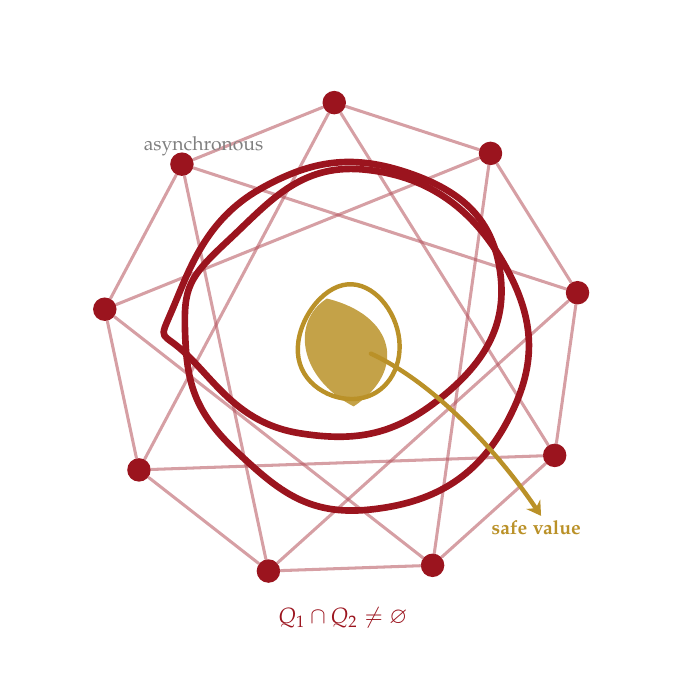
\begin{tikzpicture}[>=Stealth, line cap=round, line join=round, font=\small]
  \path[use as bounding box] (-4,-4) rectangle (4,4);

  % Network nodes
  \foreach \name/\ang in {p1/92,p2/132,p3/172,p4/212,p5/252,p6/292,p7/332,p8/12,p9/52} {
    \node[circle, fill=cmjcrimson, inner sep=3pt] (\name) at (\ang:3.05) {};
  }

  % Network edges - improved visibility
  \foreach \a/\b in {p1/p2,p2/p3,p3/p4,p4/p5,p5/p6,p6/p7,p7/p8,p8/p9,p9/p1,p1/p4,p2/p5,p3/p6,p4/p7,p5/p8,p6/p9,p7/p1,p8/p2,p9/p3} {
    \draw[cmjnetwork, line width=1.1pt, opacity=0.55] (\a) -- (\b);
  }

  % First quorum region (Q1) - darker, more visible
  \draw[cmjcrimson, line width=2.4pt, line join=round]
    plot[smooth cycle, tension=0.82] coordinates {
      (-2.15,0.45) (-1.05,1.95) (0.85,2.15) (2.00,0.90)
      (1.25,-0.70) (-0.55,-1.15) (-1.95,-0.18)
    };

  % Second quorum region (Q2) - darker, more visible
  \draw[cmjcrimson, line width=2.4pt, line join=round]
    plot[smooth cycle, tension=0.82] coordinates {
      (-1.45,1.30) (0.25,2.20) (2.05,1.00) (2.08,-1.02)
      (0.35,-2.12) (-1.35,-1.38) (-2.00,0.10)
    };

  % Safe value region - filled and outlined
  \fill[cmjgold!85]
    (-0.20,0.56)
    .. controls (0.66,0.35) and (0.83,-0.35) .. (0.14,-0.81)
    .. controls (-0.56,-0.45) and (-0.66,0.27) .. (-0.20,0.56);

  \draw[cmjgold, line width=1.6pt, line join=round]
    plot[smooth cycle, tension=0.94] coordinates {
      (0.00,0.73) (0.71,0.10) (0.26,-0.70) (-0.56,-0.20)
    };

  % Arrow pointing to safe value
  \draw[cmjgold, line width=1.6pt, -{Stealth[length=5pt,width=6pt]}]
    (0.36,-0.14) .. controls (1.18,-0.52) and (1.98,-1.40) .. (2.52,-2.20);

  % Labels with improved spacing and contrast
  \node[cmjgray, font=\scriptsize, anchor=west] at (-2.65,2.50) {asynchronous};
  \node[cmjgold, font=\scriptsize\bfseries, anchor=east] at (3.15,-2.35) {safe value};
  \node[cmjcrimson, font=\footnotesize\bfseries] at (0,-3.50) {$Q_1 \cap Q_2 \neq \varnothing$};

\end{tikzpicture}
\end{document}